%%%%%%%%%%%%%%%%%%%%%%%%%%%%%%%%%%%%%%%%%%%%%%%
%%%%%%%%%%%%% CONFIGURATION %%%%%%%%%%%%%%%%%%%
%%%%%%%%%%%%%%%%%%%%%%%%%%%%%%%%%%%%%%%%%%%%%%%

\documentclass[12pt,a4paper,final,makeidx]{report}
\usepackage[cm]{fullpage}
\usepackage[utf8x]{inputenc}
\usepackage{listings}
\usepackage{color}
\usepackage{textcomp}
\usepackage{graphicx}
\graphicspath{/home/thoorfr/NetBeansProjects/GeoImageViewer/doc/}
\usepackage[pdfborder={0 0 0 0}]{hyperref}

\lstset{
  language=Java,
  emphstyle=\underbar
  backgroundcolor=\color[rgb]{0.95,0.95,0.95}, % choose the background color
  tabsize=4,
  basicstyle=\scriptsize,
  upquote=true,
  aboveskip={1.5\baselineskip},
  columns=fixed,
  showstringspaces=false,
  extendedchars=true,
  breaklines=true,
  prebreak = \raisebox{0ex}[0ex][0ex]{\ensuremath{\hookleftarrow}},
  frame=single,
  showtabs=false,
  showspaces=false,
  showstringspaces=false,
  identifierstyle=\ttfamily,
  keywordstyle=\color[rgb]{0,0,1},
  commentstyle=\color[rgb]{0.5,0.55,0.5},
  stringstyle=\color[rgb]{0.1,0.5,0.1},
  identifierstyle=\textbf,
  frameround=tttt
}
\author{Francois-Xavier Thoorens}
\title{SUMO devoloper manual}

%%%%%%%%%%%%%%%%%%%%%%%%%%%%%%%%%%%%%%%%%%%%%%%%%%%%%%
%%%%%%%%%%%%%  DOCUMENT START HERE %%%%%%%%%%%%%%%%%%%
%%%%%%%%%%%%%%%%%%%%%%%%%%%%%%%%%%%%%%%%%%%%%%%%%%%%%%

\begin{document}
\maketitle
\tableofcontents



\chapter{Introduction}
%%%%%%%%%%%%%%%%%%%%%%

This manual is dedicated for the people that will develop the core functionnality of SUMO as well as plugins to the platform.
It is not meant to normal end users.
SUMO as a package is divided in 3 parts:
\begin{enumerate}
\item The Image Reader Library project called \textbf{GeoImage} (package org.geoimage)
\item The Core Platform project called \textbf{GeoImageViewer} (package org.geoimage.viewer)
\item A set of plugins, including the VDS analysis project called \textbf{GeoImageAnalysis}
\end{enumerate}
The manual will extensively describes those three parts.
It will start by describing how to set up the environment to develop SUMO, including the needed libraries



\chapter{Setting Up Your System}
%%%%%%%%%%%%%%%%%%%%%%%%%%%%%%%%

SUMO is entirely developed in JAVA. You need an IDE to be able to compile properly the project.
Build system is based on ANT, as generated by the netbeans IDE (as of today version 6.8). The source code is back up by a Subversion (SVN) repository hosted in JRC. The source is not open yet to people outside JRC.

\section{Environement Requirements}
%---------------------------------%
\subsection{Minimum}
\begin{itemize}
\item RAM: 1G
\item CPU: 1.8Ghz
\item Graphic Card: supporting OpenGL 2.0. Don't forget to update your drivers. More information at \url{http://worldwind.arc.nasa.gov/java/video.html}
\end{itemize}
\subsection{Recommended}
\begin{itemize}
\item RAM: 2G
\item CPU: dual core 1.8 Ghz
\item Graphic Card: NVidia GForce
\end{itemize}

\section{The IDE}
%---------------%
\begin{itemize}
\item Download and install the latest Java JDK, \textbf{not the JRE}, you can find at \url{http://java.sun.com}.
\item Download and install the last version of Netbeans, at the time of writing versin 6.8, check it out here \url{http://www.netbeans.org}.
You need to download the Java developer version (recommended).
\item Download and install also the \textbf{JOGL netbeans pack} you can find at \url{http://plugins.netbeans.org/PluginPortal/faces/PluginDetailPage.jsp?pluginid=3260}.
\item if you are on linux system, be sure you have subversion installed (most of the time it is present by default).
On Ubuntu the command is \textit{sudo apt-get install subversion}.
For windows, Netbeans has a plugin that is automatically installed the first time you decide to check out a subversion repository.
You may also use your own one like \textbf{Tortoise SVN}.
\end{itemize}
You may use Eclipse IDE as well, since the build system is based on ANT, but you will have to find out manually how to bing JOGL in Eclipse.

\section{Checking out the Subversion Repository}
%----------------------------------------------%
On netbeans 6.8 in the go to \textbf{team $>$ subversion $>$ checkout}.
The "check out" URL is \url{https://ipsc-trac.jrc.it/subversion/fish}.
Use the login/password you have to log to the JRC email system since the Suversion repository is using LDAP for authentication.
If you have problem with failed authentication, please contact the ipsc-trac.jrc.it administrator (at the time of writing \textbf{francesco.storti@ext.jrc.ec.europa.eu}).
Leave other parameters blank.
In the next step, checkout out the the four following projects:
\begin{enumerate}
\item trunk/sumo/trunk/GeoImage
\item trunk/sumo/trunk/GeoImageViewer
\item trunk/sumo/trunk/GeoImageAnalysis
\end{enumerate}
Leave other parameters as default.
\begin{quote}
There are some extra projects in trunk/sumo/trunk that are plugins you may checkout later.
\end{quote}
Netbeans proceed to the check out. It will ask to open automatically the projects. Answer yes.

\section{Configuring your project}
%--------------------------------%
The libary you needs are downloaded from the SVN. However you have to properly link the libraries in your project:
\subsection{Setting your OS}
Also it is JAVA, the JOGL library is using native libraries and need to know your default OS.
In the project.properties file you can find in GeoImageViewer/nbproject/project.properties, navigate to \textbf{natives.platform} and set the values properly: \textbf{linux-i586} or \textbf{windows-i586}.
Other OS are also suported, please refer to JOGL Netbeans Pack manual.

\subsection{Geotools}
In the project properties (\textbf{right click on the project $>$ properties}) switch to library tabs and add a new Library you name Geotools.
Add the jars contained in GeoImageViewer/lib/geotools-2.5.1/.
\subsection{Other Libraries}
Open your GeoImageViewer/nbproject/project.properties file and be sure that the following variables are set correctly:\\
\begin{tiny}
file.reference.commons-beanutils-bean-collections.jar=lib/commons-beanutils-bean-collections.jar\\
file.reference.commons-beanutils-core.jar=lib/commons-beanutils-core.jar\\
file.reference.commons-beanutils.jar=lib/commons-beanutils.jar\\
file.reference.commons-collections-3.1.jar=lib/commons-collections-3.1.jar\\
file.reference.commons-digester-1.8.jar=lib/commons-digester-1.8.jar\\
file.reference.commons-fileupload-1.2.1.jar=lib/apache/commons-fileupload-1.2.1/lib/commons-fileupload-1.2.1.jar\\
file.reference.commons-logging.jar=lib/commons-logging.jar\\
file.reference.commons-net-2.0.jar=lib/apache/commons-net-2.0/commons-net-2.0.jar\\
file.reference.commons-net-ftp-2.0.jar=lib/apache/commons-net-2.0/commons-net-ftp-2.0.jar\\
file.reference.dsn.jar=lib/javamail-1.4.1/lib/dsn.jar\\
file.reference.FengGUI-src.zip=lib/FengGUI-src.zip\\
file.reference.FengGUI.jar=lib/FengGUI.jar\\
file.reference.gekmllib.jar=lib/gekmllib.jar\\
file.reference.georss-rome-0.9.8.jar=../GeoImage/lib/georss/georss-rome-0.9.8.jar\\
file.reference.georss-rome-src-0.9.8.jar=../GeoImage/lib/georss/georss-rome-src-0.9.8.jar\\
file.reference.h2-1.2.121.jar=lib/h2-1.2.121.jar\\
file.reference.imap.jar=lib/javamail-1.4.1/lib/imap.jar\\
file.reference.mail.jar=lib/javamail-1.4.1/mail.jar\\
file.reference.mailapi.jar=lib/javamail-1.4.1/lib/mailapi.jar\\
file.reference.pop3.jar=lib/javamail-1.4.1/lib/pop3.jar\\
file.reference.RepositoryManager.jar=../RepositoryManager/dist/RepositoryManager.jar\\
file.reference.rome-0.9.jar=../GeoImage/lib/georss/rome-0.9.jar\\
file.reference.smtp.jar=lib/javamail-1.4.1/lib/smtp.jar\\
file.reference.worldwind.jar=lib/worldwind.jar\\
...\\
javac.classpath=\
\${libs.JOGL.classpath}:\textbackslash \\
\${libs.GLUEGEN-RT.classpath}:\textbackslash \\
\${reference.GeoImage.jar}:\textbackslash \\
\${reference.GeoImageAnalysis.jar}:\textbackslash \\
\${libs.Geotools.classpath}:\textbackslash \\
\${libs.swing-app-framework.classpath}:\textbackslash \\
\${libs.absolutelayout.classpath}:\textbackslash \\
\${libs.swing-layout.classpath}:\textbackslash \\
\${file.reference.commons-beanutils-bean-collections.jar}:\textbackslash \\
\${file.reference.commons-beanutils-core.jar}:\textbackslash \\
\${file.reference.commons-beanutils.jar}:\textbackslash \\
\${file.reference.commons-collections-3.1.jar}:\textbackslash \\
\${file.reference.commons-digester-1.8.jar}:\textbackslash \\
\${file.reference.commons-logging.jar}:\textbackslash \\
\${file.reference.FengGUI-src.zip}:\textbackslash \\
\${file.reference.FengGUI.jar}:\textbackslash \\
\${file.reference.gekmllib.jar}:\textbackslash \\
\${file.reference.worldwind.jar}:\textbackslash \\
\${file.reference.mail.jar}:\textbackslash \\
\${file.reference.dsn.jar}:\textbackslash \\
\${file.reference.imap.jar}:\textbackslash \\
\${file.reference.mailapi.jar}:\textbackslash \\
\${file.reference.pop3.jar}:\textbackslash \\
\${file.reference.smtp.jar}:\textbackslash \\
\${file.reference.commons-net-2.0.jar}:\textbackslash \\
\${file.reference.commons-net-ftp-2.0.jar}:\textbackslash \\
\${file.reference.commons-fileupload-1.2.1.jar}:\textbackslash \\
\${file.reference.georss-rome-0.9.8.jar}:\textbackslash \\
\${file.reference.georss-rome-src-0.9.8.jar}:\textbackslash \\
\${file.reference.rome-0.9.jar}:\textbackslash \\
\${file.reference.h2-1.2.121.jar}\\
\end{tiny}
If your computer does not have enough RAM you may change as well:\\
\textbf{run.jvmargs=-Xmx1024m}\\
to a value like -Xmx512m



\chapter{GeoImage Library}
%%%%%%%%%%%%%%%%%%%%%%%%%%

This is the basic underlying library able to access different satellite formats. The supported formats are:
\begin{itemize}
\item Envisat Images and ERS2 (same format)
\item Radarsat1 (CEOS format)
\item Radarsat2
\item Terrasar-X
\item Cosmo-Skymed
\item A subset of Geotiff images
\end{itemize}
%\includegraphics[angle=90,width=160mm,height=230mm]{ImageLayer.png}
\section{The interface GeoImageReader}
%--------------------------------%
The main class handling the image is the interface \textbf{GeoImageReader} presenting a common API for all formats:
\lstinputlisting{../../GeoImage/src/org/geoimage/GeoImageReader.java}

The basic instructions to read images is:
\begin{lstlisting}[language=Java]
GeoImageReader gir=GeoImageReaderFactory.create("path/to/file");
\end{lstlisting}

Notice the method called \textbf{dispose()}.
It is very uncommon to use disposable objects in JAVA but this method is useful to free the System, dereferencing all instances of objects contianed in the file.
This way the garbage collector is more efficient.

You may also implement your custom image reader (for new satellite sensors for instance) implementing the \textbf{GeoImageReader} interface and adding the class name to the static array GeoImageReaderFactory.FORMATS.
You will need to recompile the library.
An externalisation of the implementation classes is foreseen.
The abstract class \textbf{SarImageReader} implements common methods of the \textbf{GeoImageReader} interface.
you may extends this class for faster implementation:
\begin{lstlisting}[language=Java]
import org.geoimage.SarImageReader

public abstract class MyImage extends SarImageReader {
  public int getNBand() {
    // code here
  }
  public String getFormat() {
    // code here
  }
  public int getNumberOfBytes() {
    // code here
  }
  public int getType(boolean oneBand) {
    // code here
  }
  public String getAccessRights() {
    // code here
  }
  public String[] getFilesList() {
    // code here
  }
  public boolean initialise() {
    // code here
  }
  public void setFile(File imageFile) {
    // code here
  }
  public int[] readTile(int x, int y, int width, int height) {
    // code here
  }
  public int read(int x, int y) {
    // code here
  }
  public String getBandName(int band) {
    // code here
  }
  public void setBand(int band) {
    // code here
  }
  public void preloadLineTile(int y, int height) {
    // code here
  }
}
\end{lstlisting}

\section{}



\chapter{GeoImageViewer}
%%%%%%%%%%%%%%%%%%%%%%%%

\section{Introduction}
%--------------------%
The User Interface to deal with the satellite images is managed by the GeoImageViewer project.
It also contains a plugin architecture in order to allow third part jars to contribute to the UI.

\section{Achitecture}
%-------------------%
The architecure is a pure SWING (the native Java User Interface toolkit) application binded with JOGL.
JOGL is a native port of OpenGL using native library for different OS.
Netbeans JOGL plugin as installed according to the manual is dealing automatically with the OS you use, if you have setup your \textbf{natives.platform} properly. 
The platform has been designed in order to let developer to contribute to the UI adding menu and panel.

\begin{figure}
\begin{center}
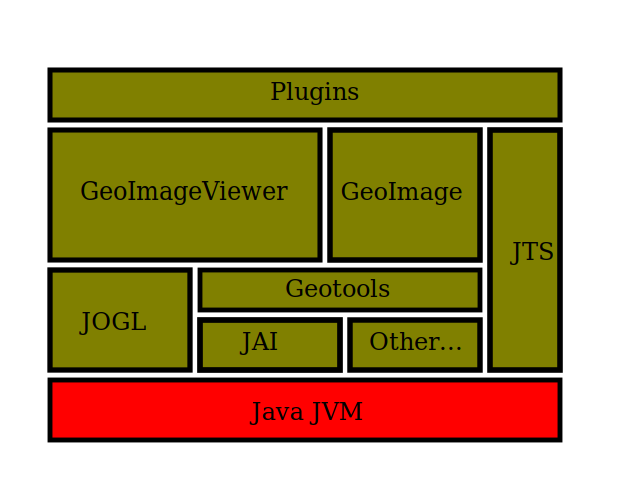
\includegraphics[width=100mm]{./images/architecture.png}
\caption{The overall architecture of GeoImageViewer and its depedencies}
\end{center}
\end{figure}

\section{API}
%-----------%
The API is contained in package \textbf{org.geoimage.viewer.core.api}.
The following classes are part of the API:

\begin{tabular}{ | l | p{10cm} | }
\hline
Argument & Class to deal with arguments passed to a plugin \\
\hline
Attributes  & Class to deal with attributes associated to a geometry \\
\hline
GeoContext  & Class containing the context of the current frame \\
\hline
GeometricLayer  & The main class backing the vector model displayed over the raster\\
\hline
IClickable  & Interface that will enable a ILayer to pass click events \\
\hline
IComplexVDSVectorLayer  & Interface that will enable an \textbf{ILayer} to be dealt as a VDS layer \\
\hline
IComplexVectorLayer  &  Interface that will enable a ILayer to be dealt as a Complex Vector Layer, ie mixing several \textbf{GeometricLayer}s \\
\hline
IConsoleAction  & Interface implemented by any class to register a plugin \\
\hline
IEditable  & Interface that will enable an \textbf{ILayer} to be notified of editing events (dragging, delete etc...) \\
\hline
IImageLayer  & Interface to enable an \textbf{ILayer} to be treated as contributing to the raster and containing several sublayers \\
\hline
IKeyPressed  & Interface that will enable an \textbf{ILayer} to be notified of keyboard events \\
\hline
ILayer  & Generic Interface of a Layer that can be displayed as such in the UI \\
\hline
ILayerListener  & Interface to listen to an \textbf{ILayer} activity \\
\hline
IListenerUser  & Interface to be notified by a \textbf{ILayer} activity \\
\hline
IMouseDrag  & Interface that will enable an \textbf{ILayer} to be notified of dragging events \\
\hline
IMouseMove  & Interface that will enable an \textbf{ILayer} to be notified of mouse movements events \\
\hline
ISave  & Interface that will enable an \textbf{ILayer} to be notified of save events \\
\hline
ISelect  & Interface that will enable an \textbf{ILayer} to be notified of select events \\
\hline
IThreshable  & Interface that will enable an \textbf{ILayer} to be notified of Thresholding events (passing a the threshold value) \\
\hline
ITime  & Interface that will enable an \textbf{ILayer} to be notified of ITime events (passing the current timespan) \\
\hline
IVectorLayer  & Interface that will enable an \textbf{ILayer} to be trated as contributing to the Vector display \\
\hline

\end{tabular}


\section{plugins}
%---------------%
The Platform is shipped with a Plugin Manager in order to activate or deactivate plugins, so the whole application will stay light.
To install a new plugin, you will need to provide to the plugin manager the jar location of your plugin and the entry class that implements org.geoimage.viewer.api.IConsoleAction.
All dependent jar files that are not already in the platform lib/ folder should be put as a convention in the lib/ folder located at the same level of your plugin jar.
If you are not following this convention, you will need to update your META-INF file with the dependant libraries (Netbeans do that automatically)



\end{document}